\subsection{Penrose diagrams}
%\FloatBarrier
	We want to know the causal structure of spacetime by asking the question which points can receive signals from which other points. 
For throwing out some irrelevant information, we will know introduce the so called \textit{conformal compactification}.
%hiermit bin ich noch nicht zufrieden!!!
\parbox{\linewidth}{~}
\hfill
\parbox{0.02\linewidth}{~}
\begin{minipage}[][][c]{0.96\textwidth}
We have two spacetimes with metrics, which are related as $g'_{\mu\nu}(x)=e^{2\omega(x)}g_{\mu\nu}(x)$ with a smooth real function $\omega(x)$. Or in other words, they differ only by multiplication with a positive scalar function on spacetime. The important thing is, those metrics have the same null geodesics.
This goes not without saying, because only timelike/spacelike curves in one metric will be timelike/spacelike curves in the other, but not geodesics.
Two metrics with this kind of relation are called \textit{conformally equivalent}. 
This gives us a way to represent the asymptotic behaviour of spacetimes at large distances.
\end{minipage}
\hfill

\parbox{\linewidth}{~}%hier Abstände nicht verändern!

Now, \textit{conformal compactification} is including infinity as a boundary of spacetime in a manifold by taking a function $\omega(x)$ that diverges while we approach infinity, so that infinity is brought into a finite distance.

	\subsubsection{of Minkowski space \checkmark}
		%\clearpage		
		
	We will now show this on an example, the ordinary flat Minkowski space, whose metric in spherical coordinates looks like
		\begin{equation}
			\diff s^2=- \diff t^2+ \diff r^2+r^2 \diff \Omega^2_2
		\end{equation}
	Because the interesting things are happening in the asymptotical behavior at $r \rightarrow \infty$ and $|t| \rightarrow \infty$, we parametrize them with the aid of $\arctan(x)$, so that the boundary is pulled in a finite distance.
		\begin{equation}
		\begin{split}
			T+R\equiv\arctan(t+r) \\
			T-R\equiv\arctan(t-r)
		\end{split}
		\end{equation}
	
	And now the metrics looks as follows:
		\begin{equation} \label{TRmetric}
			\diff s^2=
			\frac{1}{\cos^2(T+R)\cos^2(T-R)}
			\left[- \diff T^2+ \diff R^2+\left(\frac{\sin(2R)}{2}\right)^2 \diff \Omega^2_2 \right].
		\end{equation}	
					
%		\begin{figure}[tbp]	
%		\begin{center}
%		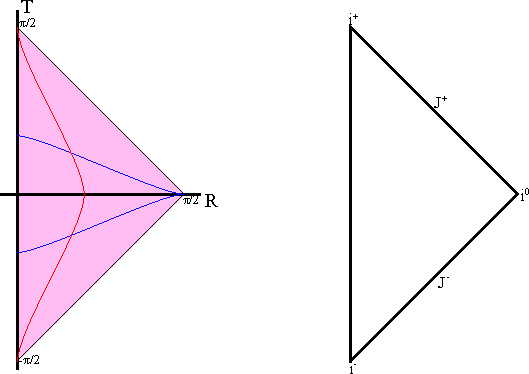
\includegraphics[scale=1]{flatpenrose}
%		\end{center}
%		\caption{On the left you see the full \textbf{Minkowski space} in pink in the RT plane. We removed the prefactor of \eqref{TRmetric}, because it would diverge at the boundary. On the right we formalize this in to a \textbf{Penrose diagram}.}\label{flatpenrose}
%		\end{figure}
	This seems to be quite complicated, but if you have a look at \textbf{Figure \ref{flatpenrose}}, you will see, why we were doing this. The new ranges of our coordinates are $|T \pm R|< \pi/2, R\geq0$, and the spacetime was compactified by including the boundary at $|T \pm R| = \pi/2$. 
	
	The new boundary which are illustrated in \textbf{Figure \ref{flatpenrose}} on the right side, is divided into five parts:	
		\begin{tabbing}
			\hspace{0.1\linewidth} \= \hspace{0.4\linewidth} \= \hspace{0.1\linewidth} \= \hfill \kill
			$i^+$~~: \> future timelike infinity \> $J^+$~~: \> future null infinity \\
			$i^-$~~: \> past timelike infinity \> $J^-$~~: \> past null infinity\\
			\hspace{0.35\linewidth} \= \hspace{0.1\linewidth} \= \hfill \kill	
			~ \> $i^0$~~: \> spatial infinity 
		\end{tabbing}
	So timelike curves come from $i^-$ and go to $i^+$, same for null curves with $J^\mp$, the spatial geodesics are ending at $i^0$. Massless particles are entering/leaving at $i^\mp$ and massive particles at $J^\mp$. The scattering matrix\footnote{also called S-matrix} maps the states on $J^- \cup i^-$ to the states on $J^+ \cup i^+$.	
	
	From this diagram, we learn that the Minkowski space does \textit{not} have \textit{event horizons}.
	%\clearpage
	\begin{figure}[tbp]	
		\begin{center}
			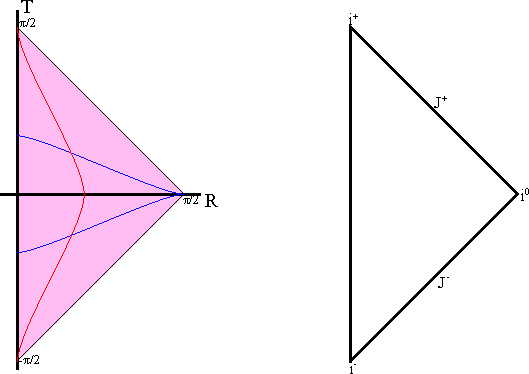
\includegraphics[scale=1]{flatpenrose}
		\end{center}
		\caption{On the left you see the full \textbf{Minkowski space} in pink in the RT plane. We removed the prefactor of \eqref{TRmetric}, because it would diverge at the boundary. On the right we formalize this in to a \textbf{Penrose diagram}.}\label{flatpenrose}
	\end{figure}
	\\ \\
	But what about the other two dimensions, the angulars i.e. the $\Sp^2$. In the Penrose diagram of the Minkowski space it is suppressed at each point. This is allowed because of the spherical symmetry of the metric \eqref{TRmetric}, so nearly no information about the spacetime is lost by this simplification. 
	
	In a Penrose diagram, there are only two ways having a boundary:
	\begin{enumerate}
		\item The $\Sp^2$ has infinite size. For example in the Minkowski case at $|T \pm R| = \pi/2$
		\item The $\Sp^2$ collapses to zero. In the Minkowski case this happens at $R=0$
	\end{enumerate}
	Within the diagram, the radius of $\Sp^2$ is also changing as we move around. 	
	
	\subsubsection{of De Sitter space \checkmark}
	\FloatBarrier
	\begin{figure}[tbp]
	 	\begin{center}
			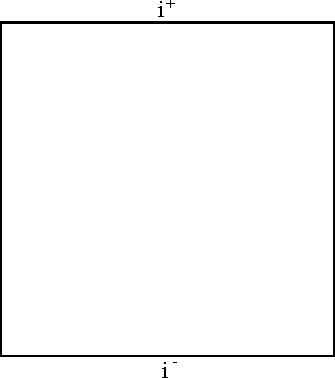
\includegraphics[scale=0.8]{dspenrose}
		\end{center}
	  		\caption{This is a Penrose diagram of the De Sitter space. As you can see, $i^{\pm}$ are spacelike surfaces instead of points like in \textbf{Figure \ref{flatpenrose}}.}\label{dspenrose}
	\end{figure}
	As we already know from \eqref{de-sitter}, the metric of the De Sitter space looks like
		\begin{equation}
			\diff s^2=- \diff \tau^2+\cosh^2\tau \diff \Omega^2_3
		\end{equation}
	As we can see in \textbf{Figure \ref{dspenrose}}, the De Sitter space has nether an infinite spatial boundary $i^0$, nor any light-like infinity $J^\mp$. That means, it is impossible to find a formulation of De Sitter space in quantum theory or an S-matrix since existing well-defined theories of quantum gravity needs either of these. 
		
	But it has \textit{event horizons}: on the left and right boundaries in \textbf{Figure \ref{dspenrose}} the $\Sp^3$ shrinks to zero size, while it goes to infinite size at $i^{\pm}$. This means, observers, who are moving on timelike geodesics at vertical straight lines in the diagram \textbf{Figure \ref{dspenrose}} could be unable to communicate.
	 
	%\FloatBarrier
	\subsubsection{of Schwarzschild geometry \checkmark}
	
	For the Penrose diagram of the Schwarzschild geometry, we take the Kruskal Szekeres coordinates of \eqref{SchXT}. That lightens the compactification we need for the Penrose diagram a lot, because the difference between $(T,X,\Omega)$ coordinates and the Minkowski space coordinates $(t,r,\Omega)$ is just their range.\footnote{Minkowski: $-\infty < t < \infty, r\geq 0$; Kruskal: $X^2-T^2 > -1$}
	So the transformation is as it was for Minkowski space:
		\begin{equation}
			\begin{split}
			T'+X'\equiv \arctan(T+X) \\
			T'-X'\equiv \arctan(T-X)
			\end{split}		
		\end{equation}
	So before we had the diamond\footnote{Here the diamond is just the geometrical shape which looks like a diamond also called rhombus.} $|R \pm T| < \pi/2$ and threw out the $R=0$ region. If this is not clear, then have a look again at \textbf{Figure \ref{flatpenrose}} for the first one. If you could add $R<0$, then you would have a diamond instead of the triangle. But instead we now have the coordinate range of $|X'\pm T'|< \pi/2$ while throwing out $|T'| > \pi/4$. The final Kruskal diagram can be seen in \textbf{Figure \ref{schpenrose}}. You can imagine two additional triangles on top and at the bottom of it, which would be the regions we cut out.
	
		\begin{figure}[tbp]  	
	  	\begin{center}
		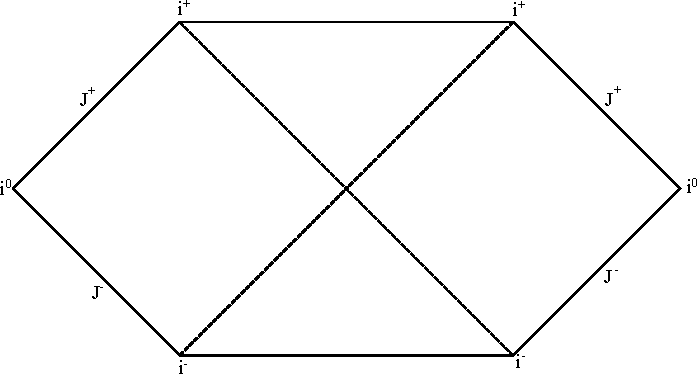
\includegraphics[scale=1]{schpenrose}
		\end{center}
		\caption{This is the \textbf{Penrose diagram} for the \textbf{Schwarzschild geometry}. The horizons are marked in dashed lines. As you can see, there are boundaries like the ones of the Minkowski space on both sides. In this diagram, the spacetime boundaries are marked explicitly with dashed lines. } \label{schpenrose}
		\end{figure}
	\FloatBarrier

